%!TEX root = Thesis_main.tex

\chapter{Controller}
\label{chapter5}

\section{Introduction and Aim of the controller}

In this chapter the core of the developed controller will be presented. The goal of our research is to solve the mobile manipulation problem of trajectory tracking for movimentation and grasping tasks. The tasks we wish to perform are in general solved decoupling the controller in order to move the mobile robot in a defined position in order to have a fixed position of the base during grasping and to reduce uncertanties in end-effector position. This approach is generally reliable since controlling indipendently the base of the robot and the arm with well known techniques allows precision and robustness. Anyway, if we want to perform the tasks in a time optimal way this approach is not suitable. The possibility to move within an enviroment during grasping operation to allow faster performance time is a goal desired not only in manipulation tasks but for many applications. Futhermore, the usage of a unique controller could allow to exploit the many degrees of redundancy to optimize other process variables such as manipulablity or obstacle avoidance capability. What we've developed, is a unique controller able to deal with the whole mobile manipulator system. The controller we developed aim to solve some of the issues presented in \ref{chapter4} by means of a Nonlinear Model Predictive Control with a novel approach to solve the online optimization problem reducing the overall computational time. The choice of MPC controller has been made for many reasons: 

\begin{itemize}
\item By means of the Reciding Horizon Principle (\ref{section_MPC}) it is possible to forecast the behaviour of the system. This approach becomes useful for obstacle avoidance and in manipulability maximization tasks.
\item It is an open framework that allows customized problems.
\item Introducing contraints allows to take into account feasibility set of the joint variable as well as control input limits.
\item Being an Optimal controller allows the minimization of customized parameters such as manipulability, control input effort etc...
\item It is generally used as a high level controller, the low level loops are in charge to track given high level command and deal with system dynamic.
\end{itemize}

In the next section will be explained the general NMPC structure for the mobile manipulation problem referring to a nonholomic vehicle and a 6 DOF's manipulator. Novel approach to reduce computational time and stability proof will be discussed later on.

\section{Problem Definition}

In this section the variables of the system and the model used for the MPC problem definition will be defined. The choice of the kinematic model instead of the dynamic one has been made for different reasons:

\begin{itemize}
\item Even if our approach allows to reduce computational time, the usage of the Dynamic model introduce further complexity in system propagation that slow down significantly the solving time.
\item Because the control action of the kinematic model is define as velocities, it's easy to implement velocity constraints.
\item Low level motor controllers are usually in charge to track velocities with higher frequency loops. This hierarchical approach is widly diffuse in controlling complex robotic systems.
\item From a user point of view, kinematic variables allows a better understanding of what's appening on the real system
\end{itemize}

\subsection{Model}

The kinematic model of the mobile manipulator is given combining \ref{dirkinMM} and \ref{base_kin_mod}. In order to do that we will define the new state variable as:
\begin{equation}
\textbf{x}(t) \in \mathbb{R}^n\ \  \textnormal{s.t.}\ \  \textbf{x}  = \left[ \begin{matrix} x \\ y \\ \theta \\ \Theta_1 \\ \Theta_2 \\ \Theta_3 \\ \Theta_4 \\ \Theta_5 \\ \Theta_6 \end{matrix} \right]\ \   \textnormal{and}\ \  \textbf{u}(t) \in \mathbb{R}^m\ \ \textnormal{s.t.}\ \ \textbf{u}=\left[ \begin{matrix} v \\ \omega \\ \dot{\Theta}_1 \\ \dot{\Theta}_2 \\ \dot{\Theta}_3 \\ \dot{\Theta}_4 \\ \dot{\Theta}_5 \\ \dot{\Theta}_6 \end{matrix} \right]
\end{equation}
By means of this variables the nonlinear kinematic model of the Nonholomic mobile manipulator can be defined as:

\begin{equation}
	\dot{\textbf{x}}=f(\textbf{x},\textbf{u})
\end{equation} 
Where:
\begin{equation} \label{NLsystem}
	f(\textbf{x},\textbf{u}) = \left[ \begin{matrix}
	G(\textbf{x}) & \textbf{0} \\ \textbf{0} & I \end{matrix} \right]
\end{equation}
and G(\textbf{x}) is defined as in \ref{Gmatrix_def}:

\begin{equation}
G(\textbf{x}) =  \left[
\begin{matrix}
\cos\theta & 0 \\
\sin\theta & 0 \\
0 & 1 
\end{matrix}
\right] 
\end{equation}

\subsubsection*{Notation:}
We will use the same notation of \ref{chapter3}. Briefely recalling: $\textbf{x}_{k|i}$ is the state vector at time instant $i$ propagated starting from time instant $k$, and in the same way with $\textbf{u}_{k|i}$

\subsection{NLP definition}

As done in \ref{chapter3} we will set up a minimization problem considering a quadratic cost function in the form:
\begin{equation}
J_{k}(\textbf{x}_{k|i},\textbf{u}_{k|i})=\sum_{i=1}^{N}l(\textbf{x}_{k|i},\textbf{u}_{k|i})
\end{equation} 
Where $l(\textbf{x}_{k|i},\textbf{u}_{k|i})$ is a positive definite function dependent on the state and the control action. By including the \ref{NLsystem} and state and control feasibility boundaries the problem becomes: 

\begin{equation} \label{ourproblem_basic}
\begin{split}
		& min_{\textbf{u}_{k|i}}\ J(\textbf{x}_{k|i},\textbf{u}_{k|i}) \\
		\textnormal{s.t.}\qquad
		&\ \ \ \ \dot{\textbf{x}}=f(\textbf{x},\textbf{u}) \\
		&\ \ \ \ \textbf{x}_{k|i} \in \mathbb{X}\ \forall\ i=1,\dots,\ N  \\
		&\ \ \ \ \textbf{u}_{k|i} \in \mathbb{U}\ \forall\ i=0,\dots,\ N-1 \\
	\end{split}	
\end{equation}
where $\mathbb{X} = \lbrace \textbf{x}\in \mathbb{R}^n\ \textnormal{s.t.}\ \textbf{x}_{min}\leq\textbf{x}\leq\textbf{x}_{max} \rbrace $ is the feasible region of the state and $\mathbb{U} = \lbrace \textbf{u}\in \mathbb{R}^m\ \textnormal{s.t.}\ \textbf{u}_{min}\leq\textbf{u}\leq\textbf{u}_{max} \rbrace $.
Note that the problem has to be discretized, we will refer at $T_k$ as the discretization time, so the time between $k$ and $k+1$ as well as the time between $i$ and $i+1$.
The problem defined in \ref{ourproblem_basic} is a standard NMPC problem that can be solved using well known numerical optimization methods, where equation \ref{NLsystem} is numerically integrated to propagate the state $\textbf{x}_{k|i+1}$. Anyway the problem so defined is to find a solution $U^*\ \in\ \mathbb{R}^{mX(N-1)}\ \textnormal{s.t.}\ U^* =[\textbf{u}^*_{k|0},\ \textbf{u}^*_{k|1},\ \dots,\ \textbf{u}^*_{k|N-1}]$. Even if, according to MPC logic, only the first computed control action $\textbf{u}^*_{k|0}$ will be applied, the problem needs to be solved for all the prediction horizon. Because of that, the dimension of the problem is highly dependendt on N. Considering our case for example, we have $m=8$, so if we set $N=20$ the dimension of $U^*$ that has to be found is $8X20=160$. The dependence of the problem dimension on the optimization horizon length generate restrictions on the choice of $N$. This is due to the increase in computational time that may become too high to solve fast online applications like handling and grasping for mobile manipulators. A solution could be to bound the value of $N$ in order to keep the problem within a solvable dimension. However, some task's performance like obstacle avoidance increase as $N$ increase. For this reason we introduced a parameterized control input approach to reduce the depencende of $N$ on the solving time.

\subsection{Parameterization}

The problem defined as in \ref{ourproblem_basic} use a control action defined as picewise constant that, as explained before, brings high computational cost dependence on $N$. To solve this issue we porpose to express the control vector $\textbf{u}_{k|i}$ as a function of some parameters:
\begin{equation}\label{param_eq}
\textbf{u}_{k|i}=F(t_j)\textbf{p}_k
\end{equation}
Where $\textbf{p} \in \mathbb{R}^p$ s.t. $\textbf{p}=[\ p_1,\ p_2,\ \dots,\ p_{N_p}\ ]$ and $F(t_j)$ is the matrix of the base of the new space $R^p$. The parameters  A good choice of the parameterization is made according to the phisics of the variables to be parameterized. In \cite{kelly2013mobile} a parametric optimal approach is proposed, anyway, given that the variables to be controlled are longitudinal and angular velocities, a polynomial parameterization can fit the phisical meaning requirement. A better explanation of how to choose the parameterization will be given in \ref{stabproof}.

\begin{figure}[h!]
	\centering
	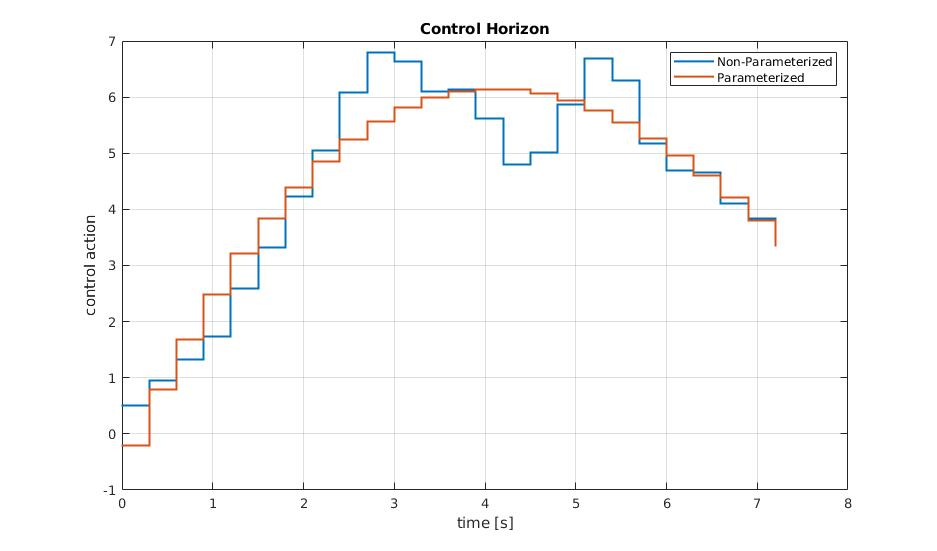
\includegraphics[scale=0.4]{param_horizon}
	\caption{Control input parameterization}
	\label{param_horizon}
\end{figure}
Considering a 3rd order Polynomial parameterization as in \ref{param_horizon} we have that each control input (i.e. each raw of the $\textbf{u}$ vector) can be expressed as a function of four parameters, for example $v=p_1i^3+p_2i^2+p_3i+p_4$.
More in general $\textbf{u}_{k|i}$ is
\begin{equation}
\textbf{u}_{k|i}=\left[ \begin{matrix}
H(i)          & \textbf{0} & \dots      & \textbf{0}  \\
\textbf{0} &     H(i)      & \dots      & \textbf{0}  \\
\vdots     & \vdots     & \ddots     & \vdots      \\
\textbf{0} & \dots      & \textbf{0} &   H(i)         \\
\end{matrix} \right] \left[ \begin{matrix} \textbf{p}_v \\ \textbf{p}_{\omega} \\ \textbf{p}_{\Theta_1} \\ \textbf{p}_{\Theta_2} \\ \vdots \\ \textbf{p}_{\Theta_6} \end{matrix} \right]
\end{equation}
Where: 
\begin{equation}
\left[ \begin{matrix} \textbf{p}_v \\ \textbf{p}_{\omega} \\ \textbf{p}_{\Theta_1} \\ \textbf{p}_{\Theta_2} \\ \vdots \\ \textbf{p}_{\Theta_6} \end{matrix} \right] = \left[ \begin{matrix} p_1 \\ p_2 \\ \vdots \\ p_{32} \end{matrix} \right]\ \ \textnormal{and }\ \ H(i)=[\ t_j^3\ \ t_j^2\ \ t_j\ \ 1\ ]
\end{equation}
Note that $t_j$  is defined as:
\begin{equation*}
	t_j=t_j(i)=T_k(i-1)\ \ \ \ \forall\ i=1,\dots,\ N-1
\end{equation*}
By applying the change of variables in \ref{param_eq} of the problem formulation in \ref{ourproblem_basic} we obtain: 
\begin{equation} \label{ourproblem_basic}
\begin{split}
		& min_{\textbf{p}_k}\ J(\textbf{x}_{k|i},\textbf{p}_k) \\
		\textnormal{s.t.}\qquad
		&\ \ \ \ \dot{\textbf{x}}=\tilde{f}(\textbf{x},\textbf{p},t) \\
		&\ \ \ \ \textbf{x}_{k|i} \in \mathbb{X}\ \forall\ i=1,\dots,\ N  \\
		&\ \ \ \ \textbf{p}_k\   \in \mathbb{P}\ \\
	\end{split}	
\end{equation}
Where $\mathbb{P} = \lbrace \textbf{p}\in \mathbb{R}^p\ \textnormal{s.t.}\ F(t_j(i))\textbf{p} \in \mathbb{U}\ \forall\ i = 1,\ \dots,\ N-1 \rbrace $. By means of this substitution the problem has to be minimized with respect to $N_p$ parameters, that don't depend on N. In fact, using 3rd order polinomial as proposed, we have to minimize with respect to $32$ parameters, even for large prediction horizon. Implementing this approach results in a faster solution of the optimization problem, and the possibility to enlarge significantly the prediction horizon. Anyway $N$ has to be chosen properly: increasing too much the prediction horizon may result in bad performances due to overconstraining of the control action. This effect, as well as a performance comparison with respect to traditional MPC will be discussed later on.

\subsection{Terminal constraints-free approach}

\section{Stability Proof}\label{stabproof}

\section{Constraints}

%\\ x_{ee} \\ y_{ee} \\ z_{ee} \\ \phi_{1_{ee}} \\ \phi_{2_{ee}} \\ \phi_{3_{ee}}